% =====================================================================
% Semana 3 · S3.3 — Realimentación por emisor
% Fundamentos de Sistemas Electrónicos Analógicos (Ingeniería Aeroespacial)
% Compilar: pdflatex semana_3_s33_realimentacion_emisor.tex  (2 pasadas)
% =====================================================================
\documentclass[aspectratio=169]{beamer}

\usepackage[utf8]{inputenc}
\usepackage[T1]{fontenc}
\usepackage{lmodern}
\usepackage[spanish,es-tabla]{babel}
\usepackage{amsmath,amssymb}
\usepackage{siunitx}
\usepackage{booktabs}
\usepackage{microtype}
\usepackage{circuitikz}

\definecolor{navy}{RGB}{23,54,93}
\definecolor{navysoft}{RGB}{72,101,140}
\definecolor{gold}{RGB}{179,142,62}
\definecolor{ink}{RGB}{44,51,58}
\definecolor{soft}{RGB}{244,241,234}

\usetheme{default}
\setbeamertemplate{navigation symbols}{}
\setbeamertemplate{footline}[frame number]
\setbeamercolor{structure}{fg=navy}
\setbeamercolor{frametitle}{fg=white,bg=navy}
\setbeamercolor{title}{fg=navy}
\setbeamercolor{subtitle}{fg=navysoft}
\setbeamercolor{itemize item}{fg=gold}
\setbeamercolor{itemize subitem}{fg=gold}
\setbeamercolor{block title}{fg=white,bg=navy}
\setbeamercolor{block body}{bg=soft}
\setbeamercolor{example text}{fg=navy}
\setbeamertemplate{itemize item}{\scriptsize\raise1.25pt\hbox{\donotcoloroutermaths$\bullet$}}
\setbeamertemplate{itemize subitem}{\scriptsize\raise1.25pt\hbox{\donotcoloroutermaths$\circ$}}
\setbeamerfont{frametitle}{size=\large,series=\bfseries}

\title[S3.3 · Realimentación por emisor]{Realimentación por emisor}
\subtitle{S3.3 — Simulaciones y laboratorio de la Semana 3}
\institute{Licenciatura en Ingeniería Aeroespacial\\ UNAM · ENES Unidad Juriquilla}
\author{M. en C. José de Jesús Santana Ramírez}
\date{Semestre 2027-1}

\begin{document}

% ---------------------------------------------------------------------
\begin{frame}[plain]
  \titlepage
\end{frame}

% ---------------------------------------------------------------------
\begin{frame}{Objetivos de la sesión}
  \begin{itemize}
    \item Entender la \textbf{realimentación negativa} que introduce $R_E$.
    \item Calcular el punto Q de la polarización con $R_E$ (realimentación por emisor).
    \item Ver cómo $R_E$ \textbf{reduce la sensibilidad} a $\beta$ y a la temperatura.
    \item Comparar las tres topologías (fija, realimentación, divisor).
  \end{itemize}
  \pause
  \begin{block}{Idea}
    Si $I_C$ sube $\Rightarrow$ $V_E$ sube $\Rightarrow$ $V_{BE}$ baja $\Rightarrow$ $I_B$ baja $\Rightarrow$ $I_C$ baja.
    Esta realimentación negativa \emph{autoestabiliza} el punto Q.
  \end{block}
\end{frame}

% ---------------------------------------------------------------------
\begin{frame}{Teoría 1 · Polarización con realimentación por emisor}
  \begin{center}
    \resizebox{0.66\linewidth}{!}{%
    \begin{circuitikz}[american voltages, scale=1.0]
      \node[npn] (Q) at (4.2,1.6) {$Q$};
      \draw (0,0) to[V, l={$V_{CC}=12\,\mathrm{V}$}, i=$I$] (0,3.2);
      \draw (0,3.2) -- (7,3.2);
      \draw (0,0) -- (7,0);
      \node[ground] at (7,0) {};
      \draw (Q.C) to[R, l={$R_C=3.3\,\mathrm{k}$}] (7,3.2);
      \draw (Q.E) to[R, l={$R_E=1\,\mathrm{k}$}] (4.2,0);
      \draw (Q.B) to[R, l={$R_B=470\,\mathrm{k}$}] (1.6,1.6) -- (1.6,3.2);
    \end{circuitikz}}
  \end{center}
  \[
    I_E \approx \frac{V_{CC}-V_{BE}}{R_B/(\beta+1) + R_E}
    \qquad
    I_C = \frac{\beta}{\beta+1}\,I_E
  \]
\end{frame}

% ---------------------------------------------------------------------
\begin{frame}{Teoría 2 · Por qué se estabiliza}
  \[
    I_E \approx \frac{V_{CC}-V_{BE}}{R_B/(\beta+1) + R_E}
  \]
  \pause
  \begin{itemize}
    \item Sin $R_E$: $I_C = \beta\cdot\dfrac{V_{CC}-V_{BE}}{R_B}$ (depende linealmente de $\beta$, como la fija).
    \item Con $R_E$: el término $R_E$ domina sobre $R_B/(\beta+1)$, así que $I_C$ depende \textbf{menos} de $\beta$.
    \item $R_E$ también amortigua la variación de $V_{BE}$ con la temperatura ($\approx -2\,\text{mV}/^\circ\text{C}$).
  \end{itemize}
\end{frame}

% ---------------------------------------------------------------------
\begin{frame}{Ejercicio · Cálculo del punto Q}
  \begin{block}{Datos}
    \centering
    $V_{CC} = \SI{12}{\volt}$, $R_B = 470\,\text{k}$, $R_C = 3.3\,\text{k}$, $R_E = 1\,\text{k}$, $V_{BE} = \SI{0.7}{\volt}$, $\beta = 100$.
  \end{block}
  \[
    I_E = \frac{12-0.7}{470\,\text{k}/(101) + 1000} = \frac{11.3}{4653 + 1000} = \frac{11.3}{5653} = \SI{1.998}{\milli\ampere}
  \]
  \[
    I_C = \frac{100}{101}\,I_E \approx \SI{1.98}{\milli\ampere}
    \qquad
    V_{CE} = 12 - 1.98\,\text{mA}(3.3\,\text{k}+1\,\text{k}) = \SI{3.49}{\volt}
  \]
  \pause
  \begin{itemize}
    \item Punto Q: $(1.98\,\text{mA},\,3.49\,\text{V})$, en \textbf{activa}.
    \item Es más estable que la fija, algo menos que el divisor de base.
  \end{itemize}
\end{frame}

% ---------------------------------------------------------------------
\begin{frame}{Resultado de la simulación · Comparación de estabilidad}
  \begin{center}
    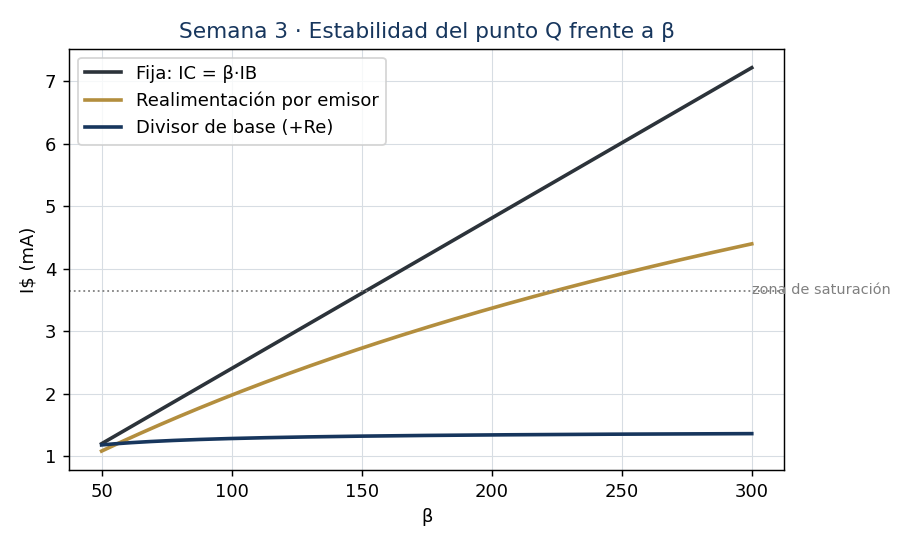
\includegraphics[width=0.72\textwidth]{figs/s3_estabilidad.png}
  \end{center}
  \begin{itemize}
    \item \textbf{Fija (gris):} $I_C$ crece linealmente con $\beta$ (inestable).
    \item \textbf{Realimentación (dorada):} pendiente intermedia.
    \item \textbf{Divisor de base (azul):} casi horizontal (la más estable).
  \end{itemize}
\end{frame}

% ---------------------------------------------------------------------
\begin{frame}{Errores comunes}
  \begin{table}
    \small
    \begin{tabular}{p{0.34\textwidth}p{0.30\textwidth}p{0.30\textwidth}}
      \toprule
      Error & Consecuencia & Corrección \\
      \midrule
      Calcular $I_B = (V_{CC}-V_{BE})/R_B$ con emisor presente & Desconocer $R_E$ & $I_E = (V_{CC}-V_{BE})/(R_B/(\beta+1)+R_E)$ \\
      Ignorar el efecto de $R_E$ sobre $V_{CE}$ & $V_{CE}$ erróneo & $V_{CE} = V_{CC}-I_C(R_C+R_E)$ \\
      Suponer $I_C = \beta I_B$ con $R_E$ & Error por factor $\beta+1$ & $I_C = \frac{\beta}{\beta+1}I_E$ \\
      Usar $V_{BE}$ fijo sin deriva & Subestimar la deriva térmica & Modelar $\approx -2\,\text{mV}/^\circ\text{C}$ \\
      \bottomrule
    \end{tabular}
  \end{table}
\end{frame}

% ---------------------------------------------------------------------
\begin{frame}{Preguntas de verificación}
  \begin{enumerate}
    \item ¿Por qué $R_E$ estabiliza el punto Q? \uncover<2->{\emph{(Realimentación negativa.)}}
    \item ¿Cuánto cambia $I_C$ al variar $\beta$ en esta topología frente a la fija?
    \item ¿Qué topología es la más estable y por qué?
      \uncover<3->{\emph{(Divisor de base: $I_E \approx (V_{th}-V_{BE})/R_E$.)}}
    \item ¿Cómo afecta la deriva de $V_{BE}$ al punto Q en cada topología?
    \item ¿Qué criterio usarías para elegir $R_E$? \uncover<4->{\emph{(Compromiso estabilidad vs ganancia/margen.)}}
  \end{enumerate}
\end{frame}

\end{document}
